%%%%%%%%%%%%%%%%%%%%%%%%%%%%%%%%%%%%%%%%%%%%%%%%%%%%%
%%% Task 1 %%%%%%%%%%%%%%%%%%%%%%%%%%%%%%%%%%%%%%%%%%
%%%%%%%%%%%%%%%%%%%%%%%%%%%%%%%%%%%%%%%%%%%%%%%%%%%%%
\task{Lifting magnet}

%%%%%%%%%%%%%%%%%%%%%%%%%%%%%%%%%%%%%%%%%%%%%%
\taskGerman{Hubmagnet}

A lifting magnet made of steel with the dimensions shown in \autoref{fig:LiftingMagnet} is to carry an iron load with a mass of 700 kg. The average field line length in the load is $l_{\mathrm{load}} = \SI{250}{\milli\metre}$, the flux-carrying cross-section $A_{\mathrm{load}}$ is $\SI{0.0095}{\metre^2}$. The winding of both coils have ${N = 300}$ turns. The magnet has a circular cross-section with a diameter of $\SI{70}{\milli\metre}$. The roughness of the surfaces of the magnet and load results in an average air gap length of $\delta = \SI{0.5}{\milli\metre}$. Neglect all leakage fluxes.





\begin{germanblock}
    Ein Hubmagnet aus Stahlguss mit den Abmessungen laut \autoref{fig:LiftingMagnet} soll eine gusseiserne Last mit einer Masse von 700 kg tragen. Die mittlere Feldlinienlänge in der Last beträgt $l_{\mathrm{load}} = \SI{250}{\milli\metre}$, der flussführende Querschnitt $A_{\mathrm{load}}$ beträgt $\SI{0,0095}{\metre^2}$. Beide Spulen haben eine Windungszahl von ${N = 300}$. Der Hubmagnet besitzt einen kreisrunden Querschnitt mit einem Durchmesser von $\SI{70}{\milli\metre}$. Durch die Rauhigkeit der Oberflächen von Magnet und Last entsteht eine mittlere Luftspaltlänge von $\delta = \SI{0,5}{\milli\metre}$. Vernachlässigen Sie Streuflüsse.
\end{germanblock}

\begin{figure}[h!]
    \centering
    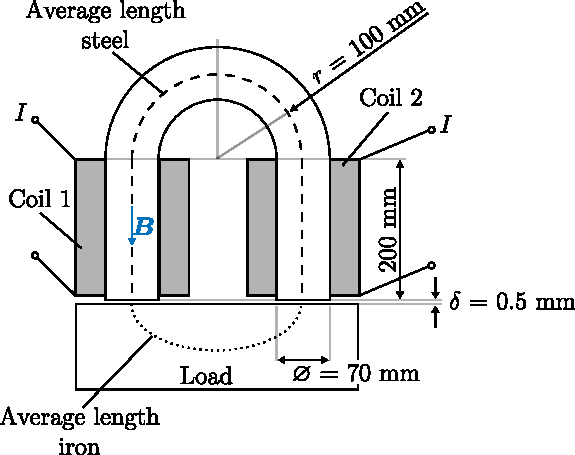
\includegraphics[width=0.6\textwidth]{fig/LiftingMagnet.pdf}
    \caption{Sketch of the lifting magnet and load with their dimensions.}
    \label{fig:LiftingMagnet}
\end{figure}



\subtask{Formulate Ampère's circuital law in the general form and in a form adapted to the magnetic circuit shown here. Use the average field line length indication as the closed curve $\partial S$.}{2}
\subtaskGerman{Stellen Sie das Durchflutungsgesetz in der allgemeinen Form und in einer der dem hier gezeigten Magnetkreis angepassten Form auf. Als geschlossene Kurve $\partial S$ verwenden Sie die mittleren Feldlinienlängen.}

\begin{solutionblock}
    The general form of Ampère's circuital law is defined as 
    $$ \oint_{\partial S} \bm{H} \cdot \mathrm{d}\bm{s} = \sum_k \theta_k$$

    with the extension to the given task:
    $$ \sum_k \theta_k = l_{\mathrm{load}} H_{\mathrm{load}} + 2 l_{\updelta} H_{\mathrm{\updelta}} + l_{\mathrm{m}} H_{\mathrm{m}}. $$
\end{solutionblock}


\subtask{Add current direction symbols of the two coils to the above figure such that they fit to the already indicated magnetic flux orientation.}{2}
\subtaskGerman{Zeichnen Sie in der Abbildung die Stromrichtung der beiden Spulen so ein, dass sich die Richtung des bereits skizzierten Magnetfeldes ergibt.}

\begin{solutionblock}
    The current direction is visualized in \autoref{fig:LiftingManet_sol_current} with red color.

    \begin{solutionfigure}[ht]
    \centering
    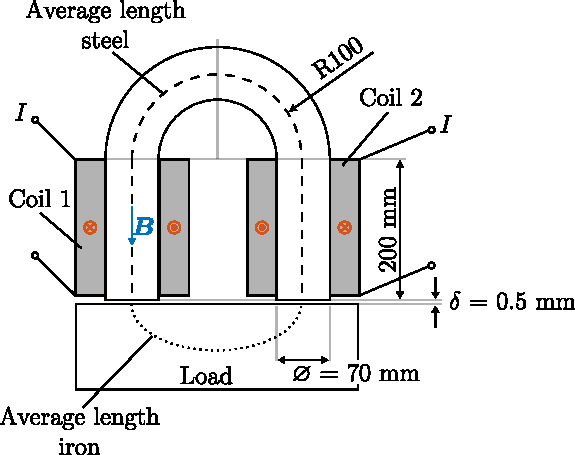
\includegraphics{fig/LiftingMagnet_sol_current.pdf}
    \caption{Necessary current direction marked in red.}
    \label{fig:LiftingManet_sol_current}
\end{solutionfigure} 
    
\end{solutionblock}

\subtask{How large is the weight force acting on the load assuming nominal gravity at sea level? Calculate the magnetic flux density in the air gap, so that the load floats straight. Use $F = \frac{B_{\updelta}^2}{2\mu_{0}}2 A_{\mathrm{m}}$ to calculate the force with $\mu_0 = 4\pi \cdot \SI{10^{-7}}{\volt \second \per \ampere \per\metre}$ being the magnetic field constant.} {2}
\begin{hintblock}
if and only if you are not able to solve this subtask, use $B_{\updelta} = \SI{1.6}{\tesla}$ as a substitute result for the following questions.
\end{hintblock}
\subtaskGerman{Wie groß ist die Gewichtskraft, die auf die Last wirkt, wenn diese auf Meereshöhe der nominellen Gravitation ausgesetzt sind? Berechnen Sie die magnetische Flussdichte im Luftspalt, so dass die Last gerade schwebt. Benutzen Sie für die Berechnung der Kraft folgende Gleichung: $F = \frac{B_{\updelta}^2}{2\mu_{0}}2 A_{\mathrm{m}}$, mit der magnetischen Feldkonstante $\mu_0 = 4\pi \cdot \SI{10^{-7}}{\volt \second \per \ampere \per\metre}$.}
\begin{germanhintblock}
nur für den Fall, dass Sie kein Ergebnis in dieser Subaufgabe berechnen können, verwenden Sie $B_{\updelta} = \SI{1,6}{\tesla}$ als Ersatzwert für die folgenden Fragen.
\end{germanhintblock}

\begin{solutionblock}
    The air gap area is calculated with
    $$ A_{\updelta} = \pi \frac{d^2}{4} = \pi \cdot \frac{\left(\SI{0.07}{\metre}\right)^2}{4} = \SI{0.0038}{\metre^2}$$

    and the weight force is definded as follwos:
    $$ F = m g = \SI{700}{\kg} \cdot \SI{9.81}{\metre\per\second^2} = \SI{6867}{\newton}.$$


    Hence, and the given equation in the task, the flux density in the air gap is determined by:
    $$ B_{\updelta} = \sqrt{\frac{\SI{6867}{\kg\metre\per\second^2}\cdot 2 \cdot 4\pi \cdot \SI{10^{-7}}{\volt \second \per \ampere \per\metre}}{2 \cdot \SI{0.0038}{\metre^2}}} = \SI{1.51}{\tesla}.$$

    
\end{solutionblock}



\subtask{How large is the necessary current $I$ for both coils to achieve this lifting task? Use the magnetization curves in \autoref{fig:magCurve}.}{3}

\subtaskGerman{Wie groß ist der benötigte Strom $I$ durch die beiden Spulen zur Realisierung des Hubs? Nutzen Sie dafür die Magnetisierungskurven in \autoref{fig:magCurve}.}


\begin{figure}[h!]
    \centering
    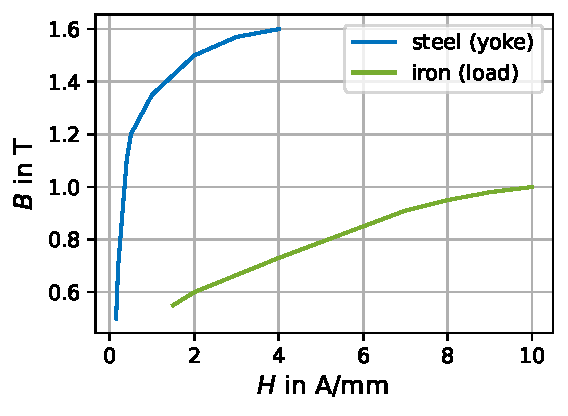
\includegraphics{fig/magCurve.pdf}
    \caption{Magnetization curves for the yoke (steel) and the load (iron).}
    \label{fig:magCurve}
\end{figure}



\begin{solutionblock}
    The given magneto static situation is represented with
    $$ N I = \sum_k \theta_k = \sum_k l_k H_k, $$
    and, therefore, the single contributions must be determined.
    Since the leakage flux is neglected, the fluxes $\phi_{\updelta}$ in the air gap and $\phi_{\mathrm{load}}$ in the iron are equal. This results into
    $$\phi_{\updelta} = \phi_{\mathrm{load}} = A_{\updelta} B_{\updelta} = A_{\mathrm{load}} B_{\mathrm{load}} $$

    thus, the magnetic flux density in the load is determined as
    $$ B_{\mathrm{load}} = \frac{A_{\updelta}}{A_{\mathrm{load}}} B_{\updelta} = \frac{\SI{0.0038}{\metre^2}}{\SI{0.0095}{\metre^2}} \cdot \SI{1.51}{\tesla} = \SI{0.60}{\tesla},$$

    and the corresponding magnetic field is $H_{\mathrm{load}} = \SI{2000}{\ampere\per\metre}$ derived from \autoref{fig:magCurve}. 

    Also, the magnetic flux in the yoke $\phi_{\mathrm{m}}$ is equal to the air gap flux, which results in
    $$ \phi_{\updelta} = \phi_{\mathrm{m}} = A_{\updelta} B_{\updelta} = A_{\mathrm{m}} B_{\mathrm{m}}, $$

    hence, the flux density is calculated with
    $$ B_{\mathrm{m}} = \frac{A_{\updelta}}{A_{\mathrm{m}}} B_{\updelta} = \frac{\SI{0.0038}{\metre^2}}{\SI{0.0038}{\metre^2}} \cdot \SI{1.51}{\tesla} = \SI{1.51}{\tesla}$$

    and the corresponding magnetic field is determined from \autoref{fig:magCurve} to $H_{\mathrm{m}} = \SI{2000}{\ampere\per\metre}$.


    The magnetic field in the air gap is calculated with the magnetic constant and the relative permeability, which is $\mu_{\mathrm{r}} \approx 1$ for air. Therefore, only the magnetic constant $\mu_{0}$ applies to:
    $$ H_{\updelta} = \frac{B_{\updelta}}{\mu_{0}} = \frac{\SI{1.51}{\tesla}}{4\pi \cdot \SI{10^{-7}}{\volt\second\per\ampere\per\metre} } = \SI{1201619}{\ampere\per\metre}.$$


    Hence, the magnetic voltage is calculated by
    \begin{align*}
    \begin{split}
        \theta &= 2 l_{\updelta} H_{\updelta} + l_{\mathrm{m}} H_{\mathrm{m}} + l_{\mathrm{load}} H_{\mathrm{load}} \\
        &= 2\cdot \SI{\frac{0.5}{1000}}{\metre} \cdot \SI{1201619}{\ampere\per\metre} + \SI{0.3142}{\metre} \cdot \SI{2000}{\ampere\per\metre} + \SI{0.280}{\metre} \cdot \SI{2000}{\ampere\per\metre} = \SI{2390}{\ampere},
    \end{split}
    \end{align*}

    which leads to the necessary current as follows:
    $$ I = \frac{\theta}{N} = \frac{\SI{2390}{\ampere}}{600} = \SI{3.98}{\ampere}.$$

    
    
\end{solutionblock}


\subtask{Determine the flux $\phi_{\mathrm{coil}}$ through one coil.}{1}
\subtaskGerman{Bestimmen Sie den Fluss $\phi_{\mathrm{coil}}$ durch eine Spule.}

\begin{solutionblock}
    The flux through one coil is calculated with:
    $$\phi_{\mathrm{coil}} = B_{\mathrm{m}} A_{\mathrm{m}} = \SI{1.51}{\tesla} \cdot \SI{0.0038}{\metre^2} =  \SI{5.74}{\milli\volt\second}.$$ 
\end{solutionblock}


\subtask{Calculate the flux linkage $\psi_{\mathrm{coil}}$ of one coil.}{1}
\subtaskGerman{Berechnen Sie den verketteten Fluss von einer Spule $\psi_{\mathrm{coil}}$.}

\begin{solutionblock}
    The flux linkage of one coil is calculated by:
    $$ \psi_{\mathrm{coil}} = N \phi_{\mathrm{coil}} = 300 \cdot \SI{5.74}{\milli\volt\second} = \SI{1.72}{\volt\second}.$$
\end{solutionblock}

